\documentclass[a4paper,12pt]{article}
\usepackage[ngerman]{babel}
\usepackage{multirow}
\usepackage{xltxtra}
\usepackage[utf8x]{inputenc}
\usepackage{fontspec}
\usepackage{eurosym}
\usepackage{amsfonts}
\usepackage{graphicx}
\usepackage[paper=a4paper,left=25mm,right=25mm,top=25mm,bottom=25mm]{geometry}
\usepackage{makecell}
\usepackage[table]{xcolor}
\usepackage{float}
\usepackage[normalem]{ulem}
\usepackage{xcolor,colortbl}
\definecolor{Gray}{gray}{0.85}
\usepackage[automark]{scrlayer-scrpage}
\usepackage[
	colorlinks=true,
	urlcolor=blue,
	linkcolor=green
]{hyperref}
\setlength{\parindent}{0em}
\setlength{\parskip}{1ex}
\pagestyle{scrheadings}
\clearscrheadfoot
\usepackage[defaultsans]{droidsans}
\renewcommand*\familydefault{\sfdefault}
\begin{document}
\input{theme.tex}
\input{version.tex}
\newcommand{\combineDivisions}{Hinweis: Wenn weniger als 5 Teams in einer der
Altersgruppen angemeldet sind, hat die Veranstaltungsleitung die Möglichkeit,
Altersgruppen zusammenzulegen. }

\newcommand{\declareExhibition}{Wenn insgesamt weniger als 5 Teams angemeldet
sind kann die Veranstaltung zur Ausstellung erklärt werden. }

\newcommand{\robotRequirements}{Autonomer Roboter, basierend auf einer
beliebigen Plattform, der \euro{1.500} oder weniger kostet und die folgenden
Designbedingungen erfüllt, die beim Check-In überprüft werden:}


\newcommand{\tournamentScoring}{
\begin{figure}[H]
	\centering
	\def\svgwidth{\columnwidth}
	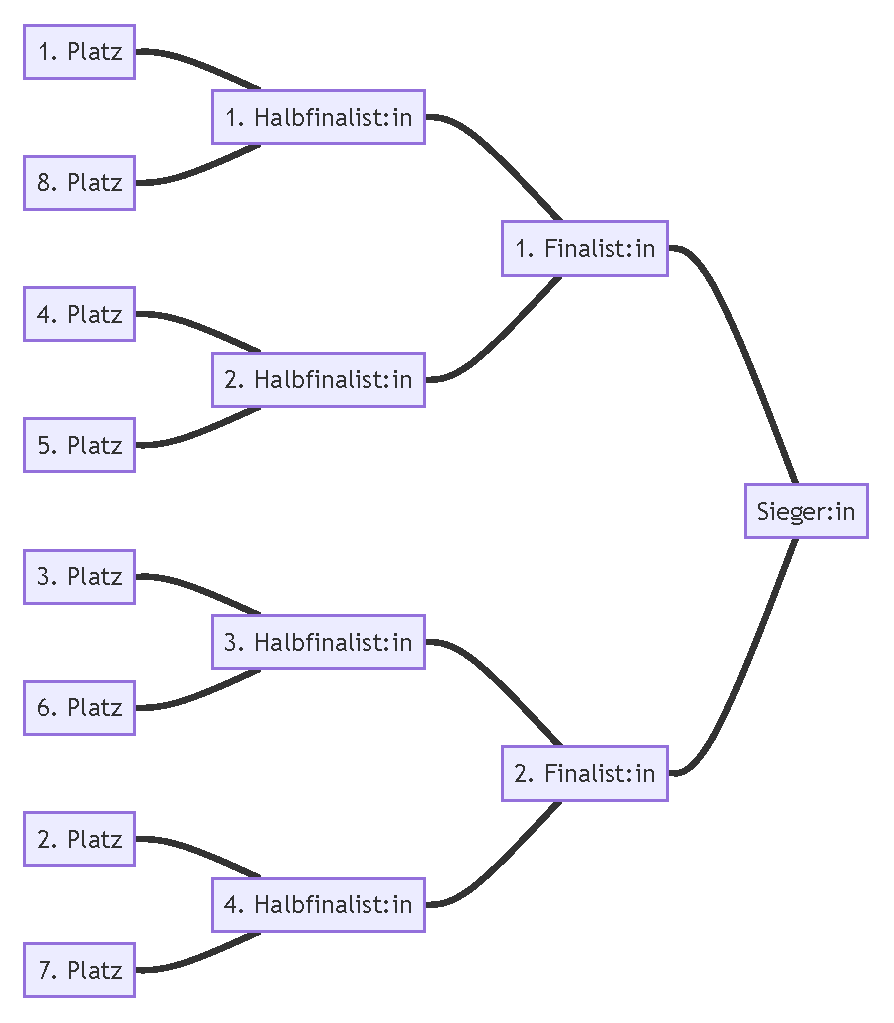
\includegraphics{tournament_score/tournament_score.pdf}
\end{figure}
}

\newcommand{\tournamentQualification}{Die aufsteigenden Teams werden
entsprechend ihrer Gesamtpunktzahl in den Turnierplan eingetragen (unten findet
ihr ein Beispiel für ein typisches Turnier mit 8 Teams). }

\newcommand{\combinedTournament}{
Hinweis: Wenn weniger als 8 Teams in allen Altersgruppen angemeldet sind, hat
die Veranstaltungsleitung die Möglichkeit, den Turnierplan entsprechend
anzupassen.
}

\newcommand{\scoreRuns}{
Die besten (8) Teams, welche am Turnier teilnehmen, werden wie folgt ermittelt:
\begin{itemize}
	\item Die Veranstaltungsleitung legt fest wieviele Läufe pro Team
		offiziell gewertet werden dürfen.
	\item Davon gehen die besten Wertungen in die Gesamtpunktzahl ein.
	\item Die Veranstaltungsleitung legt fest wieviele der offiziell
		gewerteten Läufen in die Gesamtpunktzahl eingehen.
	\item Auf Grundlage dieser Gesamtpunktzahl werden die besten Teams
		ermittelt, welche am Turnier teilnehmen.
\end{itemize}
}

\newcommand{\lightConditions}{
Die Challenge kann in Bereichen mit natürlichen Licht stattfinden, welches die
Lichtverhältnisse auf dem Spielplan verändern kann. Teams sollten darauf
vorbereitet sein, diese natürlichen Bedingungen zu meistern. }

\ohead{Regelstand: \commitDate, id: \commitID}
\title{\tagYear\ Fire Fighting Challenge Regeln}

\makeatletter
\let\inserttitle\@title
\makeatother
\begin{center}
	\rrgerLogo
	\huge                      % Schriftgröße einstellen
	\bfseries                   % Fettdruck einschalten
	\\
	\inserttitle
\end{center}

\section{Ziel}
Entwerfe, baue und programmiere einen Roboter, der die 4 zufällig platzierten
Kerzen innerhalb eines durch eine weiß-schwarze Linie umrissenen Feldes orten
und löschen kann, ohne diese zu berühren.

\section{Wer kann teilnehmen?}
Teams, die an dieser Herausforderung teilnehmen, treten in einer kombinierten
Altersgruppe an.

Hinweis: \declareExhibition

\section{Anforderungen}
\robotRequirements
\begin{itemize}
	\item Der Roboter kann demonstrieren, dass er ein Programm ausführt,
		das den Start und Stopp seines Löschsystems über einen Sensor
		steuert, der entweder mit der Kerze oder dem Kreis, auf den die
		Kerze gestellt wird, interagiert.
	\item Wenn ein Ventilator verwendet wird, darf dieser einen maximalen
		Durchmesser von $12 cm$ haben und der Roboter muss über ein
		Schutzgitter verfügen.
	\item Mehrere Sensoren und Prozessoren sind zulässig.
	\item Das Volumen des Roboter darf in seiner Startposition $65030
		cm^{3}$ nicht überschreiten.
\end{itemize}

\section{Allgemeine Spielregeln und Wertung}
\begin{itemize}
	\item \scoreRuns
	\item Der Roboter startet jeden Lauf an einer Stelle entlang der
		Grenze, die von den Punktrichter:innen bestimmt wird.
	\item Die erste Kerze ist von der Startposition des Roboters aus
		sichtbar
	\item Die übrigen Kerzen werden durch eine, zwei oder drei Wände
		geschützt um die Challenge interessanter zu gestalten. (Die
		Entscheidung welche Kerze durch Wände geschützt wird, obliegt
		der Veranstaltungsleitung). Die Teammitglieder müssen ihren
		Roboter so programmieren, dass er die Wände erkennt und die
		ungeschützte Seite findet, um die Kerze löschen zu können, ohne
		in den Kreis einzudringen, in dem sich die Kerze befindet.
		Die Kerze darf nicht über die Wand hinweg gelöscht werden (die
		Punkte werden nicht gezählt, wenn es auf diese Weise
		geschieht). Wird die Wand berührt, gibt es Punktabzug.
	\item Der Roboter hat 3 Minuten Zeit, um die 4 Kerzen zu löschen
	\item Wenn Spieler:innen den Roboter nach Beginn des Laufs berühren,
		wird die Zeit gestoppt, der Lauf abgebrochen und anhand der
		Anzahl der Kerzen gewertet, die zum Zeitpunkt der Berührung des
		Roboters bereits gelöscht waren.
	\item Offizielle Spielfelder stehen zum Üben zur Verfügung, wenn sie
		nicht von Teilnehmer:innen für einen offiziellen Lauf verwendet
		werden.
\end{itemize}

\section{Challenge Spezifikation}

\subsection{Spielfeld}
\begin{itemize}
	\item Das Spielfeld ist zwischen $2,1 m$ bis $2,5 m$ breit und $3,3 m$
		bis $3,7 m$ lang.
	\item Das Spielfeld wird durch weißes und schwarzes Klebeband
		umrandet oder entsprechend gedruckt.
	\item Die Umrandung wird mit zwei nebeneinander liegenden Linien aus
		weißem Klebeband hergestellt. Diese sind zusammen etwa $7,5 cm$
		breit. Auf die beiden weißen Linien wird mittig ein schwarzes
		(ca. $2,5 cm$ breites) Klebeband geklebt.
	\item Das Spielfeld kann auch vollständig auf weißem Hintergrund
		gedruckt werden.
	\item Kerzen und Wände werden bei jedem Lauf zufällig platziert.
\end{itemize}

\subsection{Kerzen}
\begin{itemize}
	\item Die Kerzen stehen in der Mitte weißer Kreise aus PVC-Plane, deren
		Mitte durch einen schwarzen Punkt mit einem Durchmesser von $5
		cm$ gekennzeichnet ist. Die Kerzen haben unterschiedliche Höhen
		zwischen $10 cm$ und $45 cm$.
	\item Die weißen Kreise haben einen Durchmesser von $40 cm$ und weisen
		eine $2,5 cm$ breite schwarze Linie auf, die $2,5 cm$ vom
		äußeren Rand entfernt ist.
\renewcommand{\labelitemi}{$\star$}
\renewcommand{\labelitemii}{$\checkmark$}
	\item Durch Wände verdeckte Kerzen:
	\begin{itemize}
		\item 1 Kerze - keine Wand
		\item 1 Kerze - eine Wand
		\item 1 Kerze - zwei Wände
		\item 1 Kerze - drei Wände
	\end{itemize}
\end{itemize}

\subsection{Wände}
\begin{itemize}
	\item Die Wände sind zwischen $20$ und $35cm$ breit und sind $40cm$
		hoch. Sie werden von $3,5 cm$ hohen Holzsockeln gehalten, die
		über die gesamte Breite der Wand reichen können.
\end{itemize}
\begin{center}
	Alle angegebenen Maße sind Näherungen.
\end{center}
\lightConditions
\begin{center}
\includegraphics[width=0.4\textwidth]{images/candle.jpeg}
\end{center}

\section{Wertung}
Der "`Restzeitbonus"' wird nur dann gewährt, wenn alle vier Kerzen gelöscht
sind. Andernfalls erhält das Team nur die Punkte für gelöschte Kerzen.

\section{Punktabzug}
\begin{itemize}
	\item 50\% Abzug vom Wert der Kerze, wenn
	\begin{itemize}
		\item eine Kerze vom Roboter gelöscht wird, wenn er sich
			vollständig außerhalb des Kreises befindet, aber auf
			die Kerze und nicht auf eine Wand ausgerichtet ist.
		\item während des Löschvorgangs die Kerze berührt wird
	\end{itemize}
	\item Der Löschvorgang einer angezündeten Kerze ist wie folgt
		definiert: Eintreten in den Kreis, Löschen und Verlassen des
		Kreises\ldots während dieser Zeit darf der Roboter die Kerze
		nicht berühren.
	\item Kerzen die bereits gelöscht wurden werden zu Hindernissen und
		geben somit keine Strafpunkte wenn sie nach ihrem Löschvorgang
		berührt werden.
\end{itemize}
In der nachstehenden Bewertungsmatrix findet ihr Einzelheiten darüber, wie die
Punkte während eures Laufs bewertet werden.

\section{Punktetabelle}
\begin{center}
        \begin{tabular}{|c|c|c|c|c|c|}
	\hline \cellcolor[gray]{0.9}& \multicolumn{4}{c|}{\cellcolor[gray]{0.9}Anzahl gelöschter Kerzen} & \cellcolor[gray]{0.9} \\
	\cline{2-5} \multirow{-2}{*}{\cellcolor[gray]{0.9}} & \cellcolor[gray]{0.9}1. Kerze & \cellcolor[gray]{0.9}2. Kerze & \cellcolor[gray]{0.9}3. Kerze & \cellcolor[gray]{0.9}4. Kerze & \multirow{-2}{*}{\cellcolor[gray]{0.9}\makecell{Mögliche Ge-\\samtpunktzahl}}\\
	%\cline{1-6} Außerhalb Kreis & - & - & - & - &  \multirow{3}{*}{1000}\\
        \cline{1-6} \cellcolor[gray]{0.9}\makecell{Halbe Punktzahl \\ aufgrund Abzug} & \multirow{2}{*}{50} & \multirow{2}{*}{100} & \multirow{2}{*}{150} & \multirow{2}{*}{200} &  \multirow{3}{*}{1000} \\
	\cline{1-5} \cellcolor[gray]{0.9}Volle Punktzahl & 100 & 200 & 300 & 400 & \\
        \hline \multicolumn{5}{|c|}{\cellcolor[gray]{0.9}\makecell{Zeitbonus: Die Uhr zählt von 180 Sekunden herunter und stoppt, \\ wenn der Roboter die vierte Kerze löscht.}} & 0 - 180 \\
        \hline
\end{tabular}
\end{center}

\pagebreak
\section{Tunierplan}
\begin{itemize}
        \item Die besten acht Teams werden an der Endrunde teilnehmen.
        \item \tournamentQualification
\end{itemize}
\tournamentScoring
\combinedTournament
\end{document}
